\section{\secState{R}Movement Control}\label{s:movementAutomatonTheory}

\paragraph{Idea:} The key idea is to create \emph{interface} between \emph{controlled plant} (UAS) and \emph{Avoidance Algorithm} to ensure \emph{Concept Reusability} at maximum degree.  The concept is the following:

\begin{enumerate}

    \item \emph{Interface consumes} discrete command chain and guides UAS along the \emph{desired trajectory}.
    
    \item \emph{An interface} can be used to \emph{predict trajectory} based on \emph{initial state} and future command chaining. 
\end{enumerate}


\paragraph{Frazzoli Movement Automaton:} The following paragraph strongly follows Frazzoli work \cite{frazzoli2001robust} (sec 3.1-3.5). Frazolli provided the concept of \emph{Movement Automaton} (def. \ref{def:movementAutomaton}) a specialized type of \emph{Hybrid Automaton} (eq. \ref{eq:hybridAutomaton}), the concept is taken from his works \cite{frazzoli2001robust,frazzoli2000trajectory}. Other aspects and similarities are discussed in this chapter. 


The approach was proposed to reduce the \emph{computational complexity problem} of \emph{motion planning}. The quantization of the system dynamics is done through restriction of feasible nominal system trajectories to the \emph{family of time parametrized curves}. These can be obtained by the interconnection of trajectory primitives.

\emph{Trajectory primitives} are repeatable portions of trajectory (def. \cite{frazzoli2001robust}.3.1). The trajectory primitives are interconnected by \emph{transitions} to create maneuvers (movements) (def. \cite{frazzoli2001robust}.3.3). 

By combining movements as a set of trim trajectories the trajectory can be represented as a set of discrete time bounded commands. This is summarized in the definition (def. \cite{frazzoli2001robust}.3.4) based on \emph{hybrid automaton definition} (sec. \ref{s:HybridAutomaton}).
\begin{definition}[Maneuver Automaton] A maneuver automaton over a mechanical control system $S$, with symmetry group $H$ is described by the following objects:

\begin{enumerate}
    \item A finite set of indices $Q = Q_T \cup Q_M \in \N$, where the subscript T relates to trim trajectories, and the subscript M relates to maneuvers;
    
    \item A finite set of trim trajectory parameters $\left(\bar{g},\bar{\xi},\bar{u}\right)_q$; with $q\in Q_T$.
    
    \item A finite set of maneuver parameters, and state and control trajectories $\left(T,u,\phi\right)_q$, with $q\in Q_M$.
    
    \item The maps $Previous: Q_M\to Q_T $, and, $Next: Q_M \to Q_T$ such that $Previous(q)$ and $Next(q)$ give, respectively, the index of the trim trajectories from which the maneuver $q$ starts and ends.
    
    \item A discrete state $q \in Q$.
    
    \item A continuous state, denoting the position on the symmetry group, $h \in H$.
    
    \item A clock state $\theta \in \R$, which evolves according to $\dot{\theta}=1$, and which is reset after each switch on $q$.
\end{enumerate}
\begin{note}
    It is apparent that decisions can be made about the future evolution of the system only when the system is executing a trim trajectory (that is, the discrete state is in one of the nodes in the graph). While executing a maneuver the system is committed to it and must keep executing the maneuver until its completion. As a consequence, for motion planning and control design purposes, one can concentrate the study of the evolution of the system on and between nodes.
\end{note}
\end{definition}


\paragraph{Architecture:} The Movement Automaton can be seen as a consistent hierarchical abstraction of the continuous dynamics, in sense outlined in \cite{pappas2000hierarchically}: \emph{Any sequence of movement primitives generated by the Movement Automaton results by construction in a trajectory which is executable by the full continuous system. We will give a deeper meaning to hierarchical consistency}. 

\paragraph{Optimal Path Generation:} If the maneuvers are instantaneous (i.e., the UAS can transition instantaneously between two different trim trajectories), Reduction of stronger results obtained by Dubins \cite{dubins1957curves} and Reeds \cite{reeds1990optimal} concerning optimal paths for kinematic cars on the plane (see also \cite{soueres1998optimal}). 

\paragraph{Controllability:} The systems controlled by Movement Automaton (as in \cite{lavalle1998rapidly}), is controllable according to our definition, even though it is not
small-time controllable \cite{sussmann1983lie}.

\paragraph{Other Properties:} The other properties of movement automaton, like \emph{Stability, Robustness} and other important control properties are proven in \cite{frazzoli2001robust}.


\paragraph{Example:} The \emph{example} is given in (fig. \ref{fig:movementAutomatonExampleTheory}). The \emph{States} (Barrels) are connected by \emph{Transitions} (green arrows).

\emph{Hover} is the neutral and \emph{initial} state, in this place the UAS stays on place and maintains altitude.

\emph{Forward flight} is when \emph{UAS} is flying in frontal direction with constant speed. The speed-up and slow-down are incorporated in \emph{Transition} between \emph{Hover} and \emph{Forward flight} states, and it takes some time to execute. \emph{Transitions} between Turning states and \emph{Flight forward} state are almost instant. 

\emph{Steady turn left/right} is when \emph{UAS} is flying in the frontal direction and starts steady turning left or right. 

\begin{note}
UAS in (fig. \ref{fig:movementAutomatonExampleTheory}) ignores the vertical maneuvering, and it is expected to fly on horizontal plane.
\end{note}


\begin{figure}[H]
    \centering
    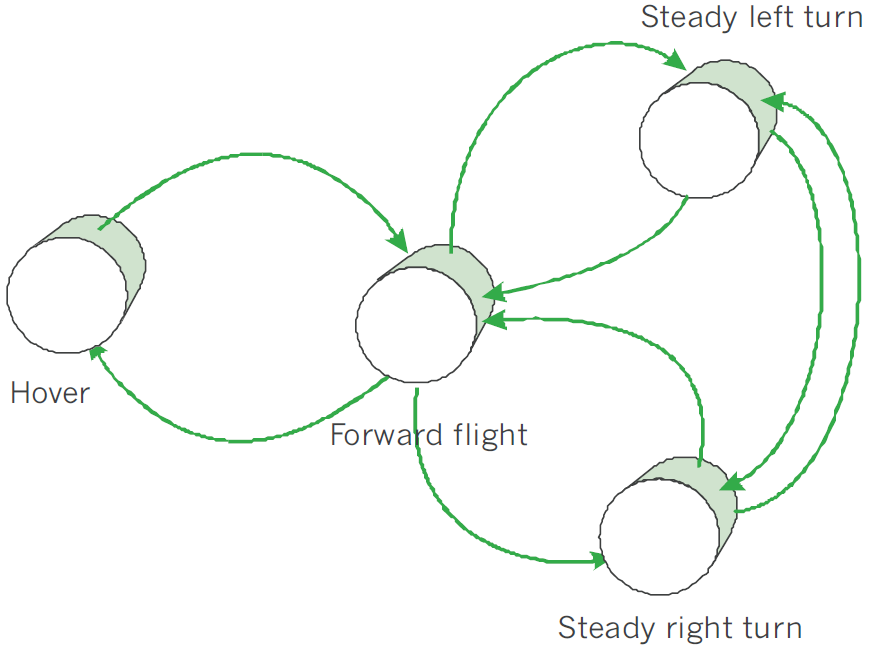
\includegraphics[width=0.55\linewidth]{\FIGDIR/TE030MovementAutomatonFrazzCite} 
    \caption{Movement Automaton for Copter UAS \cite{frazzoli2001robust}.}
    \label{fig:movementAutomatonExampleTheory}
\end{figure}

\begin{note}
The \emph{Movement Automaton} is used as with modification (sec. \ref{s:MovementAutomatonDefinitionAndProperties}). The implementation is described in (sec. \ref{s:modelMAImplementation}). The testing configuration was given in (tab. \ref{tab:testMovementOrientations}).
\end{note}

